% !TeX TXS-program:bibliography = txs:///biber

\documentclass[
    paper=a4,
    fontsize=10pt,
    DIV=12,
    % twocolumn,
    oneside,
]{scrartcl}

%___________________________________________________________________
% Imports
%-------------------------------------------------------------------------------------------------
%   Packages
%-------------------------------------------------------------------------------------------------

\usepackage[utf8]{inputenc}                         % utf8 as input encoding
\usepackage[T1]{fontenc}                            % 8bit font encdoing
\usepackage[ngerman]{babel}                         % word seperation
\usepackage{microtype}                              % font expansion
\usepackage{libertine}                              % select font
\usepackage[libertine]{newtxmath}                   % select font for mathmode
\usepackage{scrlayer-scrpage}                       % Bessere Kopfzeilen

\usepackage[
    locale=DE,
    detect-all,
    per-mode=fraction,
]{siunitx}                                          % express SI units
\usepackage{amsmath}
\usepackage{booktabs}                               % better tables
\usepackage{tabularx}                               % tables with pagewidth
\usepackage{graphicx}                               % input pictures
\usepackage{svg}
\usepackage{xcolor}
\usepackage{flushend}
\usepackage{listingsutf8}

\usepackage{csquotes}                               % quote environment
\usepackage[
    backend=biber,
    style=ieee,
]{biblatex}                                          % source control

\usepackage{hyperref}                               % add hyperlinks

%-------------------------------------------------------------------------------------------------
%   Colors
%-------------------------------------------------------------------------------------------------

% \definecolor{colorblue}{HTML}{0480CC}				% color for weblinks
% \definecolor{colordarkblue}{HTML}{4C1DCC}			% no use case at the moment
% \definecolor{colorgreen}{HTML}{26CC1B}				% color for citations
% \definecolor{colorred}{HTML}{CC1204}				% color for pdf links
\definecolor{coloryellow}{HTML}{F0B707}			    % color for warnings

%-------------------------------------------------------------------------------------------------
%   Lengths
%-------------------------------------------------------------------------------------------------

\newlength{\imagewidth}
\setlength{\imagewidth}{0.7\columnwidth}

%-------------------------------------------------------------------------------------------------
%   Style Options
%-------------------------------------------------------------------------------------------------

\KOMAoptions{
    toc     =   listof,                                     % add table of figures in 
    % headsepline=true,                               % switch header rule
    numbers =   noendperiod,
}

\hypersetup{
    colorlinks=true,
    bookmarksnumbered=true,
}

\chead{Laborbericht Regelungstechnik}
\ohead{Versuch Nr. \printlabor}
\ihead{Jan Hoegen}

\flushbottom                                        % fill pages to bottom

\addbibresource{quellen.bib}

%-------------------------------------------------------------------------------------------------
%   Macros
%-------------------------------------------------------------------------------------------------
        
\newcommand{\missing}{%
    \textcolor{coloryellow}{MISSING}%
    \PackageWarning{rtl_labor}{You used the 'missing' macro at this line. Remove it before finalising document}%
}
\newcommand{\improve}{%
    \textcolor{coloryellow}{IMPROVE}%
    \PackageWarning{rtl_labor}{You used the 'improve' macro at this line. Remove it before finalising document}%
}

\newcommand{\legend}[1]{\par\footnotesize\textbf{Legende}: #1\par}
\newcommand{\figsource}[1]{\par\footnotesize\textbf{Quelle:} #1\par}

%-------------------------------------------------------------------------------------------------
%   Title Page
%-------------------------------------------------------------------------------------------------

\titlehead{%
    Hochschule Karlsruhe\\
    University of Applied Sciences\\
    Fakultät für Elektro- und Informationstechnik
}
\title{Laborbericht Regelungstechnik}

\publishers{Betreuer: Prof. Dr. Keller}

\author{%
    Jan Hoegen\thanks{%
        Matrikel-Nr. 82358. E-Mail \href{jan.hoegen@web,de}{jan.hoegen@web,de}}%
    % \and%
    % Rithik Kurmar\thanks{%
    %     Matrikel-Nr. . E-mail \href{}{}}
}

\newcommand{\labor}[1]{\newcommand{\printlabor}{#1}}

\AtBeginDocument{
    \subtitle{Versuch Nr.~\printlabor}
    
    \hypersetup{
        pdftitle = {RT Labor \printlabor\ | Hoegen},
    }
}

%-------------------------------------------------------------------------------------------------
%   Listing Settings
%-------------------------------------------------------------------------------------------------

\lstset{%
	frame			=	tb ,							%	horizontale Linie oben&unten
	breaklines		=	true,							%	Zeilenumbruch
	rulecolor		=	\color{black} ,					%	Rahmenfarbe ist schwarz
	% keywordstyle	=	\keywordcolor ,
	% commentstyle	=	\commentcolor ,
	% stringstyle		=	\stringcolor ,
	title			=	\lstname ,						%	Titel ist gleich dem Dateinamen
	basicstyle		=	\footnotesize\ttfamily ,		%	Kleine Schrift und Monospace
	% numbers			=	right,							%	Zeilennumber rechts (da marginalie links)
	inputencoding	=	utf8,  							% Input encoding
    extendedchars	=	true,  							% Extended ASCII
}
% \lstdefinestyle{TeX}{language=TeX,						%	Mehr Keywörter für TeX
%     morekeywords={vspcae, hspace, rule, ifdefined, newcommand, setlength, newlentgh, RequirePackage, ProvidesPackage, NeedsTexFormat, DeclareOption, ProcessOption}, 
% }
\lstset{literate=							%	ermöglicht Unicode-Zeichen in Listing!
  {á}{{\'a}}1 {é}{{\'e}}1 {í}{{\'i}}1 {ó}{{\'o}}1 {ú}{{\'u}}1
  {Á}{{\'A}}1 {É}{{\'E}}1 {Í}{{\'I}}1 {Ó}{{\'O}}1 {Ú}{{\'U}}1
  {à}{{\`a}}1 {è}{{\`e}}1 {ì}{{\`i}}1 {ò}{{\`o}}1 {ù}{{\`u}}1
  {À}{{\`A}}1 {È}{{\'E}}1 {Ì}{{\`I}}1 {Ò}{{\`O}}1 {Ù}{{\`U}}1
  {ä}{{\"a}}1 {ë}{{\"e}}1 {ï}{{\"i}}1 {ö}{{\"o}}1 {ü}{{\"u}}1
  {Ä}{{\"A}}1 {Ë}{{\"E}}1 {Ï}{{\"I}}1 {Ö}{{\"O}}1 {Ü}{{\"U}}1
  {â}{{\^a}}1 {ê}{{\^e}}1 {î}{{\^i}}1 {ô}{{\^o}}1 {û}{{\^u}}1
  {Â}{{\^A}}1 {Ê}{{\^E}}1 {Î}{{\^I}}1 {Ô}{{\^O}}1 {Û}{{\^U}}1
  {ã}{{\~a}}1 {?}{{\~e}}1 {i}{{\~i}}1 {õ}{{\~o}}1 {u}{{\~u}}1
  {Ã}{{\~A}}1 {?}{{\~E}}1 {I}{{\~I}}1 {Õ}{{\~O}}1 {U}{{\~U}}1
  {œ}{{\oe}}1 {Œ}{{\OE}}1 {æ}{{\ae}}1 {Æ}{{\AE}}1 {ß}{{\ss}}1
  {u}{{\H{u}}}1 {U}{{\H{U}}}1 {o}{{\H{o}}}1 {O}{{\H{O}}}1
  {ç}{{\c c}}1 {Ç}{{\c C}}1 {ø}{{\o}}1 {å}{{\r a}}1 {Å}{{\r A}}1
  {€}{{\euro}}1 {£}{{\pounds}}1 {«}{{\guillemotleft}}1
  {»}{{\guillemotright}}1 {ñ}{{\~n}}1 {Ñ}{{\~N}}1 {¿}{{?`}}1 {¡}{{!`}}1 
  {~}{{\textasciitilde}}1 {*}{{\normalfont{*}}}1
}

% \setlength{\imagewidth}{1\columnwidth}

%___________________________________________________________________
% Title Page
\title{Laborversuch zur Drehzahlregelung}
\labor{3}
\date{\today}

%___________________________________________________________________
% Begin
\begin{document}

\maketitle

%___________________________________________________________________
% Abstract
\begin{abstract}
    \noindent    
    \subsubsection*{Abstract}
        Im dritten Regelungstechniklabor wird das Verhalten eines Elektromotors mithilfe von Matlab und SIMULINK betrachtet. Es wird ein stationär genauer Regelkreis als PI-Regler erarbeitet und sein Verhalten bei Überschwingern und zeitabhängigen Lastmomenten beobachtet.
\end{abstract}

%___________________________________________________________________
% Text

\section{Motor im Nennbetrieb}
    Die Gleichungen für den Gleichstrommotor wurden der Laboranleitung \cite{versuch3} entnommen. 
    \begin{align}
        \omega  &= 73.68 \frac{\si{\newton\meter}}{\si{\ampere\kilogram\metre\squared}} \int i \, dt\\
        i       &= \frac{1}{\SI{1e8}{\henry}} \int u - 0.028 \si{\newton\meter\per\ampere} \omega - 5 \si{\ohm} i \, dt\\
        M       &= 0.028 \si{\newton\meter\per\ampere} i
    \end{align}
    
    In SIMULINK wird das zugehöirige Blockschaltbild als Subsystem entwickelt (siehe Abbildung \ref{fig:blockMotor}) und anschließend an eine konstante Spannungsversorgung von \SI{10}{\volt} angeschlossen. Der zeitliche Verlauf der Ausgangsgrößen ist in Abbildung \ref{fig:graphMotor} dargestellt. Die Zeitkonstante \(\tau\) berechnet sich zu \SI{2.3843}{\second}.

    \begin{figure}[hbt]
        \centering
        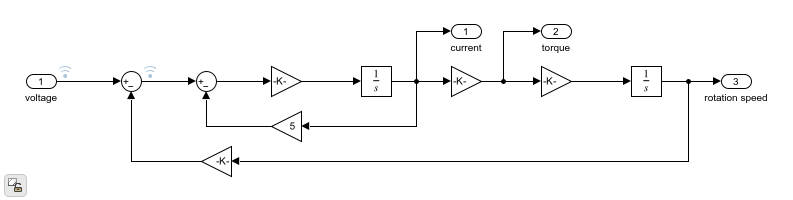
\includegraphics[width=1.3\imagewidth]{../versuch3/blockMotor}
        \caption{Blockschaltbild des Motor}
        \label{fig:blockMotor}
    \end{figure}   

    \begin{figure}[hbt]
        \centering
        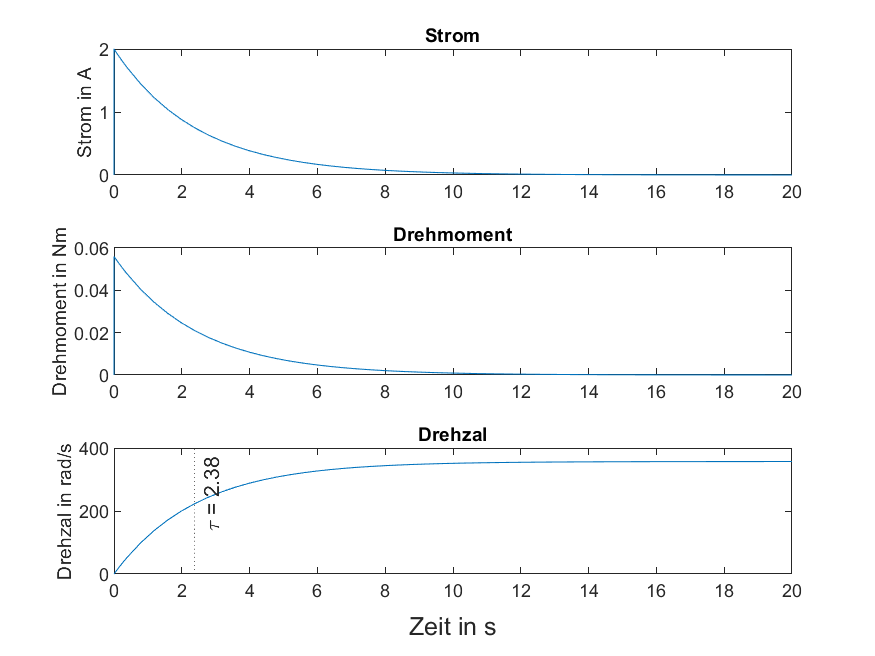
\includegraphics[width=\imagewidth]{../versuch3/graphMotorModel.png}
        \caption{Motor im Nennbetrieb}
        \label{fig:graphMotor}
    \end{figure}   

\section{Motorsteuerung mit P-Regler}
    Um die Drehzahl des Motors einzustellen wird ein P-Regler erstellt und an das Motorsubsystem angeschlossen (siehe Abbildung \ref{fig:blockPController}). Die Eingangsspannung am Motor wird mit einem Sättigungsblock in SIMULINK auf \(U_{max} = \pm \SI{10}{\volt}\) begrenzt. Die Verstärkung \(K_R\) des Reglers wird so eingestellt, dass der Sättigungsblock gerade nicht begrenzt bei einem Sollwert von \(\omega_{soll} = \SI{100}{\radian\per\second}\).
    \begin{align}
        K_R = \frac{u_{max}}{\omega_{soll}} = \frac{\SI{10}{\volt}}{\SI{100}{\radian\per\second}} = \SI{0.1}{\volt\second\per\radian}
    \end{align}

    \begin{figure}[hbt]
        \centering
        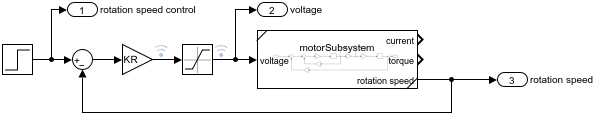
\includegraphics[width=1.3\imagewidth]{../versuch3/blockPController}
        \caption{Blockschaltbild des P-Reglers}
        \label{fig:blockPController}
    \end{figure} 

    Der zeitliche Verlauf der Reglergrößen ist in Abbildung \ref{fig:graphPController} gezeigt. Es ist zu erkennen, dass der Motor nur \(\omega_{ist} = \SI{78,1}{\radian\per\second}\) erreicht und damit nicht stationär genau ist. Das ist darin begründet, dass in diesem Zustand die Eingangsspannung am Motor 
    \begin{align}
        U = K_R \cdot (\omega_{soll} - \omega_{ist}) = \SI{0.1}{\volt\second\per\radian} \cdot \left( \SI{100}{\radian\per\second} - \SI{78.1}{\radian\per\second} \right) = \SI{2.19}{\volt}
    \end{align}
    beträgt und diese Spannung wiederum zu einer Drehzahl von \(\omega_{ist} = \SI{78,1}{\radian\per\second}\) am Motor führt.

    \begin{figure}[hbt]
        \centering
        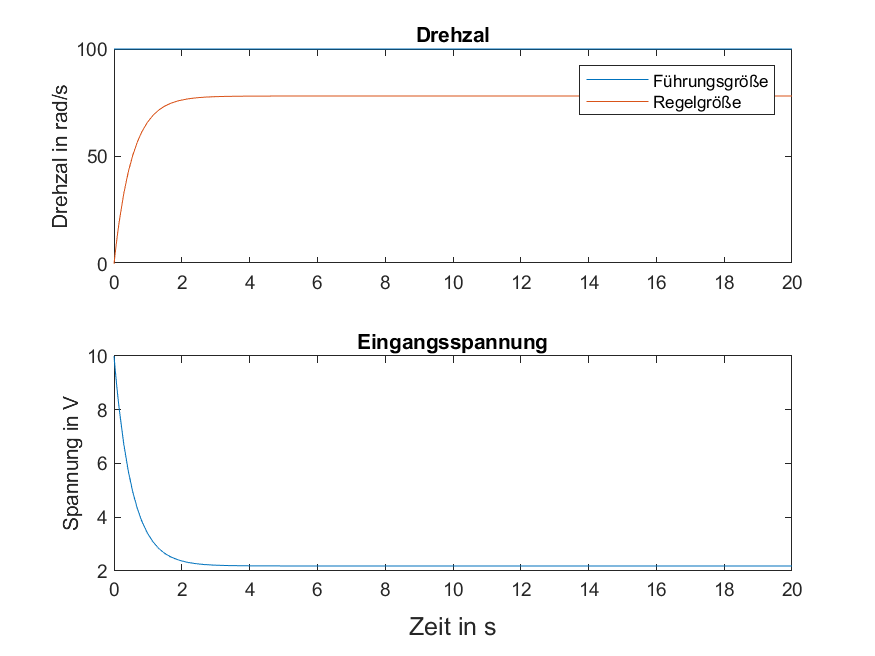
\includegraphics[width=\imagewidth]{../versuch3/graphPController}
        \caption{Reglergrößen des P-Reglers}
        \label{fig:graphPController}
    \end{figure}   

\section{Motorsteuerung mit PI-Regler}
    Der Regler aus dem vorherigen Abschnitt wird um einen Integrator erweitert (Abbildung \ref{fig:blockPiController}). Die beste Nachstellzeit \(T_N\), bei der gerade so kein Überschwinger für \(\omega_{soll} = \SI{100}{\radian\per\second}\) entsteht, wird mit einer ausgelagerten Funktion ermittelt (siehe Anhang \ref{lst:TN}). Dabei wird das Modell so lange mit veränderter Nachstellzeit aufgerufen, bis der Maximalwert der Reglergröße kleiner ist als der Sollwert. Es ergibt sich ein Wert von \(T_N = \SI{2.43}{\second}\)

    \begin{figure}[hbt]
        \centering
        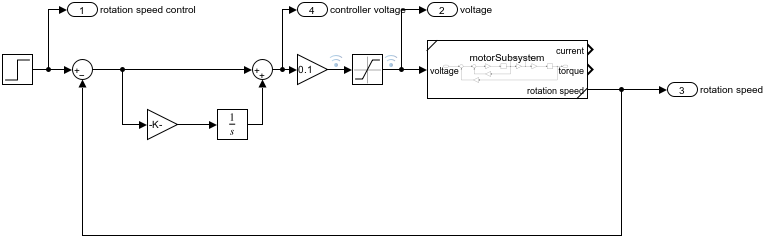
\includegraphics[width=1.5\imagewidth]{../versuch3/blockPiController}
        \caption{Blockschaltbild des PI-Reglers}
        \label{fig:blockPiController}
    \end{figure}   

    Der zeitliche Verlauf der Reglergrößen ist in Abbildung \ref{fig:graphPiController} dargestellt. Zusätzlich wird die Spannung vor und nach dem Sättigungsblock betrachtet. Wird die Führungsgröße auf \(\omega_{soll} = \SI{300}{\radian\per\second}\) angehoben (Abbildung \ref{fig:graphPiControllerNew}), kommt es zu Überschwingern. Das liegt daran, dass in der Zeit, in welcher der Begrenzer aktiv ist, sich der I-Anteil des Reglers weiter erhöht. 

    \begin{figure}[hbt]
        \centering
        \begin{subfigure}{0.49\columnwidth}
            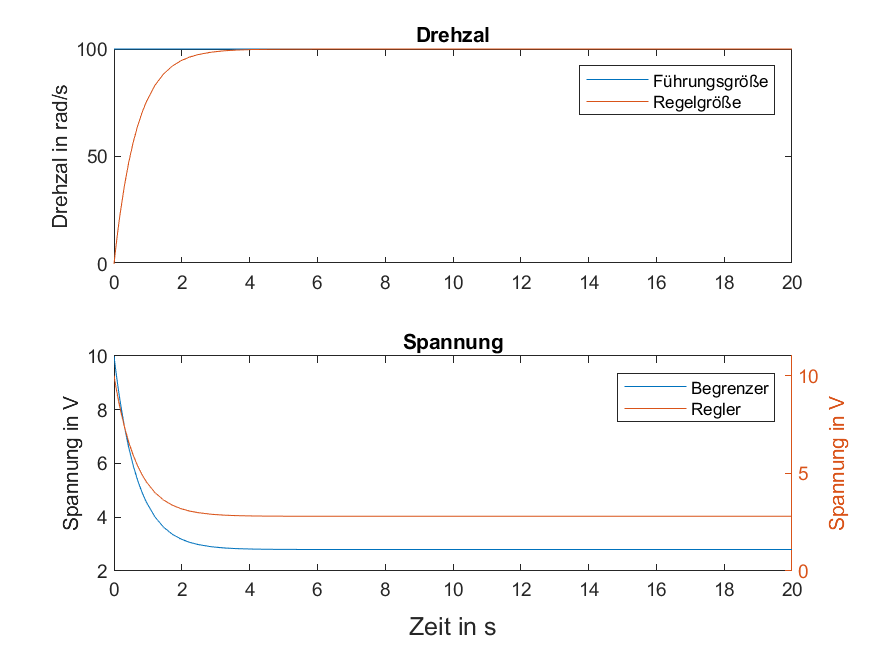
\includegraphics[width=1.0\columnwidth]{../versuch3/graphPiController.png}
            \caption{Sollwert \(\omega_{soll} = \SI{100}{\radian\per\second}\)}
            \label{fig:graphPiController}   
        \end{subfigure}%
        \hfill%
        \begin{subfigure}{0.49\columnwidth}
            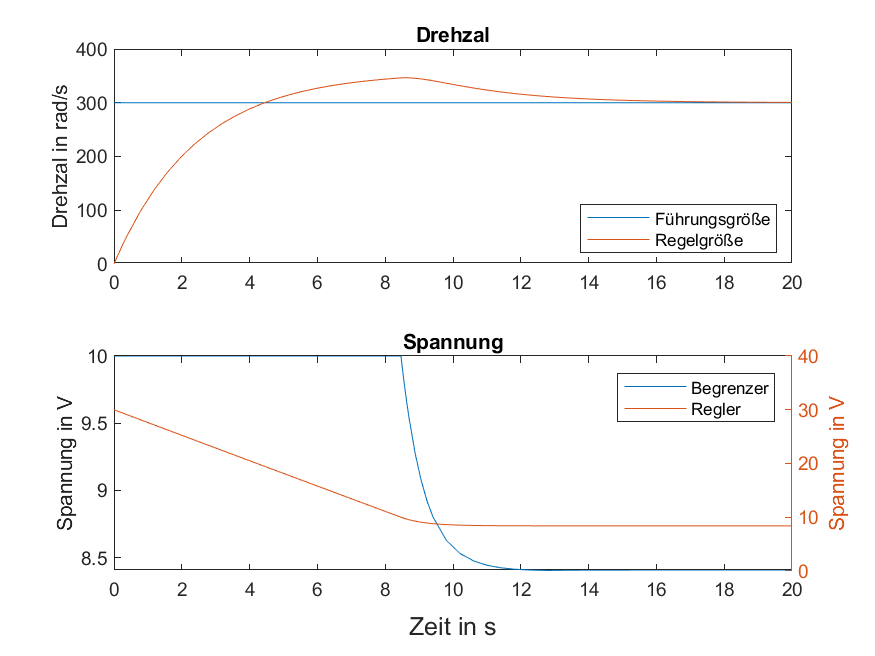
\includegraphics[width=1.0\columnwidth]{../versuch3/graphPiControllerNew.png}
            \caption{Sollwert \(\omega_{soll} = \SI{300}{\radian\per\second}\)}
            \label{fig:graphPiControllerNew}
        \end{subfigure}
        \caption{Reglergrößen des P-Reglers}
    \end{figure}

\section{Motorregelung mit veränderlichen Lastmoment}
    Nun wird ein Lastmoment, dass der Drehbewegung entgegenwirkt, nach \SI{10}{\second} hinzugeschaltet. Das erweiterte Blockschaltbild ist in Abbildung \ref{fig:blockPiControllerLoad} zu finden, das Diagramm der Reglergrößen in Abbildung \ref{fig:graphPiControllerload}. Es wurde zusätzlich das Drehmoment des Motors und das Drehmoment am Ausgang aufgezeichnet.

    \begin{figure}[hbt]
        \centering
        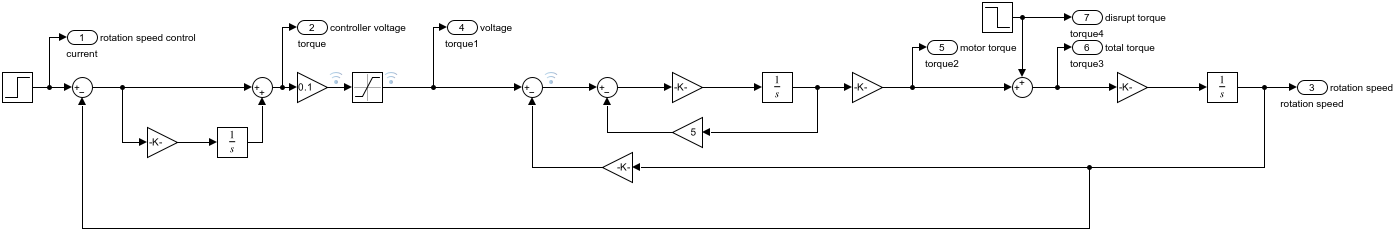
\includegraphics[width=1.7\imagewidth]{../versuch3/blockPiControllerLoad}
        \caption{Blockschaltbild des PI-Reglers mit Lastmoment}
        \label{fig:blockPiControllerLoad}
    \end{figure}

    \begin{figure}[hbt]
        \centering
        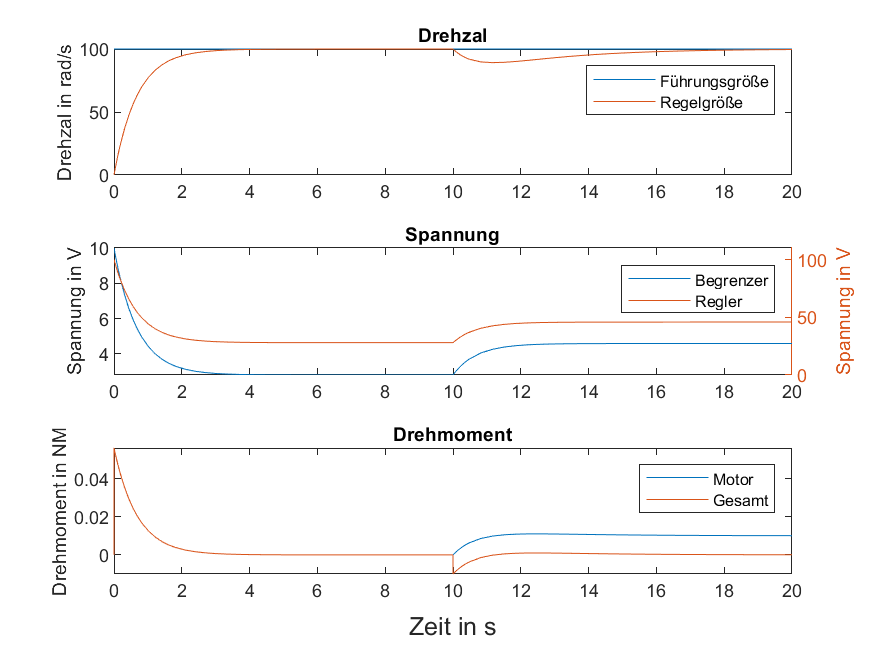
\includegraphics[width=\imagewidth]{../versuch3/graphPiControllerLoad}
        \caption{Reglergrößen des PI-Reglers mit Lastmoment}
        \label{fig:graphPiControllerload}
    \end{figure}  

%___________________________________________________________________
% End

\printbibliography[heading=bibnumbered]

\section{Autorenbeiträge}
    Maileen Schwenk und Jan Hoegen erstellten die Vorbereitung und Messauswertung. Jan Hoegen schrieb den Bericht.

\section{Verfügbarkeit des Codes}
    Der Code zum Auswerten der Daten und Erstellen der Diagramme findet sich unter \url{https://github.com/JaxRaffnix/Regelungstechnik}. Ebenfalls ist hier der Code zum Erstellen dieser Ausarbeitung hinterlegt.

%___________________________________________________________________
% Appendix
\appendix   

\section{MATLAB-Code zur Modellauswertung}
    \lstinputlisting[language=MATLAB, label={lst:}]{../versuch3/plotMotorModel.m}
    \lstinputlisting[language=MATLAB, label={lst:}]{../versuch3/plotPController.m}
    \lstinputlisting[language=MATLAB, label={lst:}]{../versuch3/plotPiController.m}
    \lstinputlisting[language=MATLAB, label={lst:}]{../versuch3/plotPiControllerLoad.m}
    \lstinputlisting[language=MATLAB, label={lst:TN}]{../functions/BestResetTime.m}
    \lstinputlisting[language=MATLAB, label={lst:}]{../functions/TimeConstantIndex.m}

\end{document}